\documentclass[11pt]{article}
\usepackage{geometry} 
\geometry{margin=1in} 
\usepackage{fullpage,amsthm,amsfonts,amssymb,epsfig,amsmath,times,amsthm,mathtools,enumitem,amsmath,graphicx}
\usepackage{pgfplots}
\usepackage{diagbox}
\usepackage{tikz-qtree}
\usepackage[retainorgcmds]{IEEEtrantools}


\title{CMPS 142 - Homework 4}
\author{Emily Hockel - echockel@ucsc.edu\\Christopher Hsiao - chhsiao@ucsc.edu}
\date{May 29, 2017} 

\begin{document}
\maketitle

\section{Determine Support Vectors}

\begin{center}
\begin{tikzpicture}
\begin{axis}[
    axis lines = left,
    xlabel = $x_1$,
    ylabel = $x_2$,
    xmin = -0.5, xmax = 2.5,
    ymin = -0.5, ymax = 2.5
]
\addplot[only marks, color=blue, mark=+]coordinates{(1,1) (1,2) (2,1)};
\addplot[only marks, color=red, mark=o]coordinates{(0,0) (1,0) (0,1)};
\addplot[domain=-0.5:2.5]{1.5 - x};
\end{axis}
\end{tikzpicture}
\end{center}

By observing the plot, we see that the support vectors are:

\begin{align*}
     x^{(1)} & = \begin{bmatrix} 1 \\ 1 \end{bmatrix}, y^{(1)} = +1 \\
    x^{(2)} & = \begin{bmatrix} 0 \\ 1 \end{bmatrix}, y^{(2)} = -1 \\
    x^{(3)} & = \begin{bmatrix} 1 \\ 0 \end{bmatrix}, y^{(3)} = -1 \\
\end{align*}
   

We use the formula $y^{(i)}(w \cdot x^{(i)} + b) = 1$ to find the maximum margin separating plane. We solve for $w$ and $b$ to find $x_2 = 1.5 - x_1$, where $w = \begin{bmatrix} 2 \\ 2 \end{bmatrix}$ and $b = -3$.

We use the formula $\frac{y^{(i)}(w \cdot x^{(i)} + b)}{||w||}$ to find that the geometric margin for the support vectors is $\frac{\sqrt{2}}{4}$.


\section{Support Vector Machine Kernels}

For each of the following problems, we used 10-fold cross validation.

\subsection{RBF Kernel}

	\begin{center}
        \begin{tabular}{ |c|c|c|c|c|c| } 
             \hline
             \diagbox{C}{$\gamma$} &  0.01 & 0.1 & 1 & 10 \\
             \hline
             0.1 & 73.1363 & 87.5027 & 89.3719 & 64.2469\\
             \hline
             1 & 87.2202 & 92.3712 & 93.0667 & 85.1771\\
             \hline
             10 & 92.1539 & 93.6753 & 93.2189 & 85.8726\\
             \hline
             100 & 93.3493 &	93.8926 & 92.5668 & 85.8292\\
             \hline
             1000 & 93.5884 & 93.4362 & 91.4584 & 85.6336\\
             \hline
        \end{tabular}
        \end{center}
        
        We see that the values $C = 1000$ and $\gamma = 0.01$ give us the highest accuracy of 93.59\%. For this data set, a narrow gaussian and a high margin penalty give us the best results.
        
\subsection{Polynomial Kernel}

        \begin{center}
        \begin{tabular}{ |c|c|c|c|c| } 
             \hline
             \diagbox{C}{$\gamma$} &  0.01  & 1 & 10 & 100\\
             \hline
             0.1 &&&&\\
             \hline
             1 & & 81.1997 & 91.2193 &\\
             \hline
             10 & & 87.394 & 92.7842 & 91.9365\\
             \hline
             100 & 60.5955 & 91.2193 & 92.4364 & 91.2628\\
             \hline
             1000 & && 91.9365 &\\
             \hline
        \end{tabular}
        \end{center}
        
        With this different kernel, we get just slightly lower accuracy than the RBF kernel. Parameter values of $C = 100$ and $\gamma = 10$ gives us an accuracy of 92.44\%. 
        
\subsection{Linear SVM}

        \begin{center}
        \begin{tabular}{ |c|c| } 
             \hline
             C & \\
             \hline
             0.1 & 85.1989\\
             \hline
             1 & 90.3282\\
             \hline
             10 & 92.2408\\
             \hline
             100 & 92.9363\\
             \hline
             1000 & 93.0233\\
             \hline
             10000 & 92.9363\\
             \hline
        \end{tabular}
        \end{center}

	With a linear SVM, we get our highest accuacy of 93.02\% with a value of $C = 1000$.
\pagebreak
\section{Greedy Decision Trees}
We built a dataset based on the logical statement:
\begin{equation}
(A \land B) \lor (\neg A \land C)
\end{equation}
\subsection{The Dataset}
Note that the last entry in the dataset has been repeated to demonstrate the pitfalls of the greedy top-down decision tree generation algorithm.
\begin{center}
        \begin{tabular}{ |c|c|c|c| } 
             \hline
             A & B & C & label\\
             \hline
             0 & 0 & 0 & $-$\\
             \hline
             1 & 0 & 0 & $-$\\
             \hline
             0 & 1 & 0 & $-$\\
             \hline
             0 & 0 & 1 & $+$\\
             \hline
             1 & 1 & 0 & $+$\\
             \hline
             1 & 0 & 1 & $-$\\
             \hline
             0 & 1 & 1 & $+$\\
             \hline
             1 & 1 & 1 & $+$\\
             \hline
             1 & 1 & 0 & $+$\\
             \hline
        \end{tabular}
\end{center}
\subsection{The Optimal Tree}
First, let us take a look at the optimal decision tree.
\begin{center}
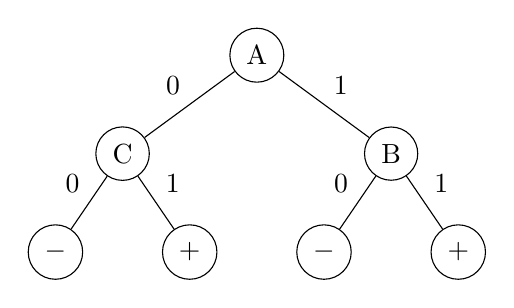
\begin{tikzpicture}[every tree node/.style={draw,circle},
   level distance=1.25cm,sibling distance=1cm,
   edge from parent path={(\tikzparentnode) -- (\tikzchildnode)}]
\Tree[.A 
	\edge node[auto=right] {$0$};
		[.C 
			\edge node[auto=right] {$0$};
			$-$
			\edge node[auto=left] {$1$};
			$+$ ]
	\edge node[auto=left]{1};
		[.B
			\edge node[auto=right] {$0$};
			$-$
			\edge node[auto=left] {$1$};
			$+$ ]]
	
\end{tikzpicture}
\end{center}
This tree has seven nodes, with four leaf nodes representing the predictions.
\subsection{The Greedy Top-Down Tree}
For the first iteration of the algorithm, let us see the split for each of the three attributes.\\
Note that we are using the error rate function, which is the fraction of predictions that are \textbf{not} in the majority of predicted values.\\

\subsubsection{First Iteration Predictions}
Below, we have the first iteration predictions and error rates for each attribute value.
\begin{itemize}
\item \textbf{A = 0}: $\{-, -, +, +\}$, error: $\frac{2}{4}$
\item \textbf{A = 1}: $\{-, -, +, +, +\}$, error: $\frac{2}{5}$
\item \textbf{B = 0}: $\{-, -, -, +\}$, error: $\frac{1}{4}$
\item \textbf{B = 1}: $\{-, +, +, +, +\}$, error: $\frac{1}{5}$
\item \textbf{C = 0}: $\{-, -, -, +, +\}$, error: $\frac{2}{5}$
\item \textbf{C = 1}: $\{-, +, +, +\}$, error: $\frac{1}{4}$
\end{itemize}

\noindent The total error across the three attributes are:
\begin{center}
\textbf{A} = $0.9$; \textbf{B} = $0.45$; \textbf{C} = $0.65$
\end{center}
Since \textbf{B} has the lowest error, we'll choose \textbf{B} as our attribute to split on.
\subsubsection{Second Iteration Predictions: Split on B}
Now, we find the second iteration predictions and error rates for the remaining attribute values \textbf{A} and \textbf{C}.
\begin{itemize}
\item \textbf{B = 0; A = 0}: $\{-, +\}$, error: $\frac{1}{2}$
\item \textbf{B = 0; A = 1}: $\{-, -\}$, error: $0$
\item \textbf{B = 1; A = 0}: $\{-, +\}$, error: $\frac{1}{2}$
\item \textbf{B = 1; A = 1}: $\{+, +, +\}$, error: $0$
\item \textbf{B = 0; C = 0}: $\{-, -\}$, error: $0$
\item \textbf{B = 0; C = 1}: $\{+, -\}$, error: $\frac{1}{2}$
\item \textbf{B = 1; C = 0}: $\{-, +, +\}$, error: $\frac{1}{3}$
\item \textbf{B = 1; C = 1}: $\{+, +\}$, error: $0$
\end{itemize}
\noindent The total error across the two attributes are:
\begin{center}
\textbf{A} = $1$; \textbf{C} = $0.83$
\end{center}
Since \textbf{C} has the lowest error, we'll choose \textbf{C} as our attribute to split on. Note that we split on both branches of \textbf{B}, so we create two \textbf{C} nodes.
\subsubsection{The Final Iteration}
This is what the tree now looks like, after the second iteration:
\begin{center}
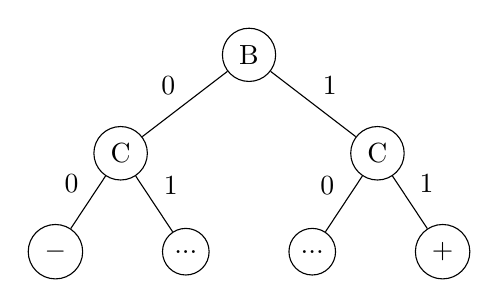
\begin{tikzpicture}[every tree node/.style={draw,circle},
   level distance=1.25cm,sibling distance=1cm,
   edge from parent path={(\tikzparentnode) -- (\tikzchildnode)}]
\Tree[.B 
	\edge node[auto=right] {$0$};
		[.C 
			\edge node[auto=right] {$0$};
			$-$
			\edge node[auto=left] {$1$};
			$...$ ]
	\edge node[auto=left]{1};
		[.C
			\edge node[auto=right] {$0$};
			$...$
			\edge node[auto=left] {$1$};
			$+$ ]]
\end{tikzpicture}
\end{center}
Now all that is left is to add the splits on \textbf{A}, for the last four sequences:
\begin{center}
\{B = 0; C = 1; A = 0\} = $+$\\
\{B = 0; C = 1; A = 1\} = $-$\\
\{B = 1; C = 0; A = 0\} = $-$\\
\{B = 1; C = 0; A = 1\} = $+$
\end{center}	

Adding these last few nodes to our tree, we get the full decision tree:
\begin{center}
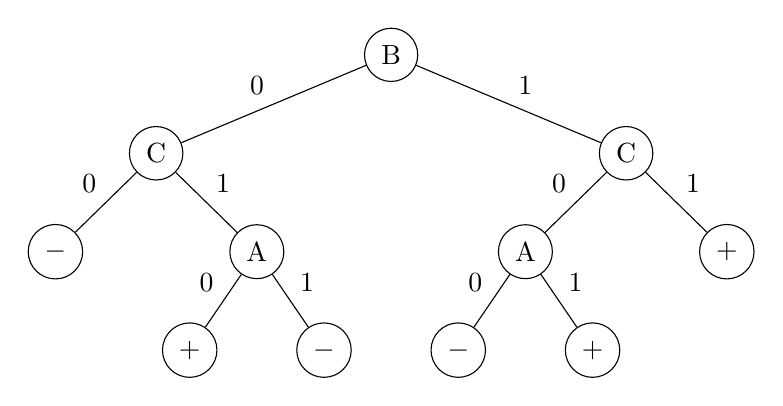
\begin{tikzpicture}[every tree node/.style={draw,circle},
   level distance=1.25cm,sibling distance=1cm,
   edge from parent path={(\tikzparentnode) -- (\tikzchildnode)}]
\Tree[.B 
	\edge node[auto=right] {$0$};
		[.C 
			\edge node[auto=right] {$0$};
			$-$
			\edge node[auto=left] {$1$};
			[.A
				\edge node[auto=right] {$0$};
				$+$
				\edge node[auto=left] {$1$};
				$-$ ]]
	\edge node[auto=left]{1};
		[.C
			\edge node[auto=right] {$0$};
			[.A
				\edge node[auto=right] {$0$};
				$-$
				\edge node[auto=left] {$1$};
				$+$ ]
			\edge node[auto=left] {$1$};
			$+$ ]]
\end{tikzpicture}
\end{center}
This is the decision tree output by the greedy top-down algorithm. This tree has $11$ nodes, and $6$ leaf nodes.\\
Recall from \textbf{3.2} that the optimal tree has $7$ nodes, with $4$ leaf nodes. Clearly, this tree is not optimal.
\end{document}